\section{Methodology}\label{sec:methods}
% Mention the overall goal of our work to keep the big picture in mind
The overall goal of our work is to improve mutlilabel classification performance of the original homepage2vec model \cite{homepage2vec}. 
We refer to this model as \texttt{baseline}. 
We can divide our work into two main phases: (1) obtaining high-quality annotations and (2) fine-tuning the baseline model with the obtained annotations. 
In the following, we describe the methodology for each phase in detail.

\subsection* {Phase 1: Obtaining High-Quality Annotations}
In the first phase, we aim to obtion hight-quality GPT annotations measuring performance against human annotatated data.
The orignal human labaled data comprises of 840 websites, anotated each by 3 diffrent annotators. 
The measured inter-anotator agreement measured by the pairwise Cohen's kappa \cite{cohen-coef} is $0.2 \pm 0.02$, indicating low agreement. 
We assign a category label if at least 2 annotators agree, resulting in an average of $2.5$ labels per website.

For 761 websites that were reachable at the time of writing we scraped their content, extracting features such as top-level domain, domain, title, description, keywords, first 50 links, and first 100 sentences, the same features used in the original Homepage2vec model \cite{homepage2vec} and we used the same pipiline for feature embedding.
Also not all features were available for all websites, as shown in Table \ref{tab:feature_information}.
\begin{table}[!ht]
\centering
\caption{Percentage of websites with each feature accross our datasets.}
\label{tab:feature_information}
\begin{tabular}{lrr}
\toprule
 & Original & Curlie-gpt-10k \\
\midrule
n & 761.00 & 9190.00 \\
tld (\%) & 100.00 & 100.00 \\
domain (\%) & 100.00 & 100.00 \\
tags (\%) & 93.69 & 95.47 \\
titles (\%) & 98.42 & 98.28 \\
descriptions (\%) & 54.93 & 62.95 \\
keywords (\%) & 19.58 & 27.29 \\
links (\%) & 89.88 & 91.62 \\
sentences (\%) & 99.08 & 99.03 \\
\bottomrule
\end{tabular}
\end{table}


This scraped pre-prcessed data is then used to obtain the annotaions using Open-AI API.
The system prompt tells the model to perform a mutlilabel classification (the full prompr can be found in the Appendix \ref{app:prompt}) and to respod in a JSON format with key value pairs representing the category and the binary classification. Additionaly one example can website with the correct label is provided to the model, making it a texttt{1-shot} classificaion.
In the user promept we provided a JSON of the exctrated features, we considered 3 different contexts given to the model, accrding to features important found in the original paper \cite{homepage2vec}. 
The smallest context \texttt{context1} includes the least amount of information about the website, making the classification faster and cheaper as less tokens are used and the \texttt{context3} having all the information about the website that was scraped.

We also considered two versions of the GPT model an older GPT-3.5 model and a newer GPT-4 model, where the GPT-4 model is more expensive and slower to use.
All variants of the Labelers can be found in Tabel \ref{tab:labelers_setup}
% - introduce labelers (parameter dimensions), introduce prompt, one shot example:
\begin{table}[htbp]
    \centering
    \begin{tabular}{lll}
        \toprule
        \textbf{Parameter} & \textbf{Variants} & \textbf{Description} \\
        \midrule
        \texttt{context} 
            & \texttt{context1} & Uses the \texttt{tld}, \texttt{domain}, and \texttt{metatags} \\
            
            & \texttt{context2} & Same as \texttt{context1} plus \texttt{title}, \\ & & \texttt{description} and \texttt{keywords} \\
            
            & \texttt{context3} & Same as \texttt{context2} plus \texttt{links} and \\ & & \texttt{text}\\

        \addlinespace
        \texttt{model} 
            & \texttt{gpt3.5} & Uses GPT-3.5 (\texttt{gpt-3.5-turbo-1106}) \\
            
            & \texttt{gpt4}   & Uses GPT-4 (\texttt{gpt-4-1106-preview}) \\
        
        \addlinespace
        \texttt{fewshot} 
            & \texttt{fewshot} & Injects an example website and label into \\ & & the system prompt \\
            
            & \texttt{zeroshot} & Does not inject any example website or \\ & & label into  the system prompt \\
        \bottomrule
    \end{tabular}
    \caption{Description of Parameters and Variants}
    \label{tab:parameters}
\end{table}

\textbf{Curlie-10k} 
We employ the best-performing GPT annotator evaluated against the human annotated original crowdsourced data to annotate \texttt{curlie-10k}, a dataset with 10k randomly selected websites from Curlie. 
Following the same preprocessing and feature extraction as the original dataset, Table \ref{tab:feature_information} displays feature percentages across datasets. 
As the figure clearly indicates, the most useful features according to the homepage2vec \cite{homepage2vec} descriptions and keywords are missing in around 55 \% and 75 \% of cases, respectively. 

\begin{figure}[!ht]
    \centering
    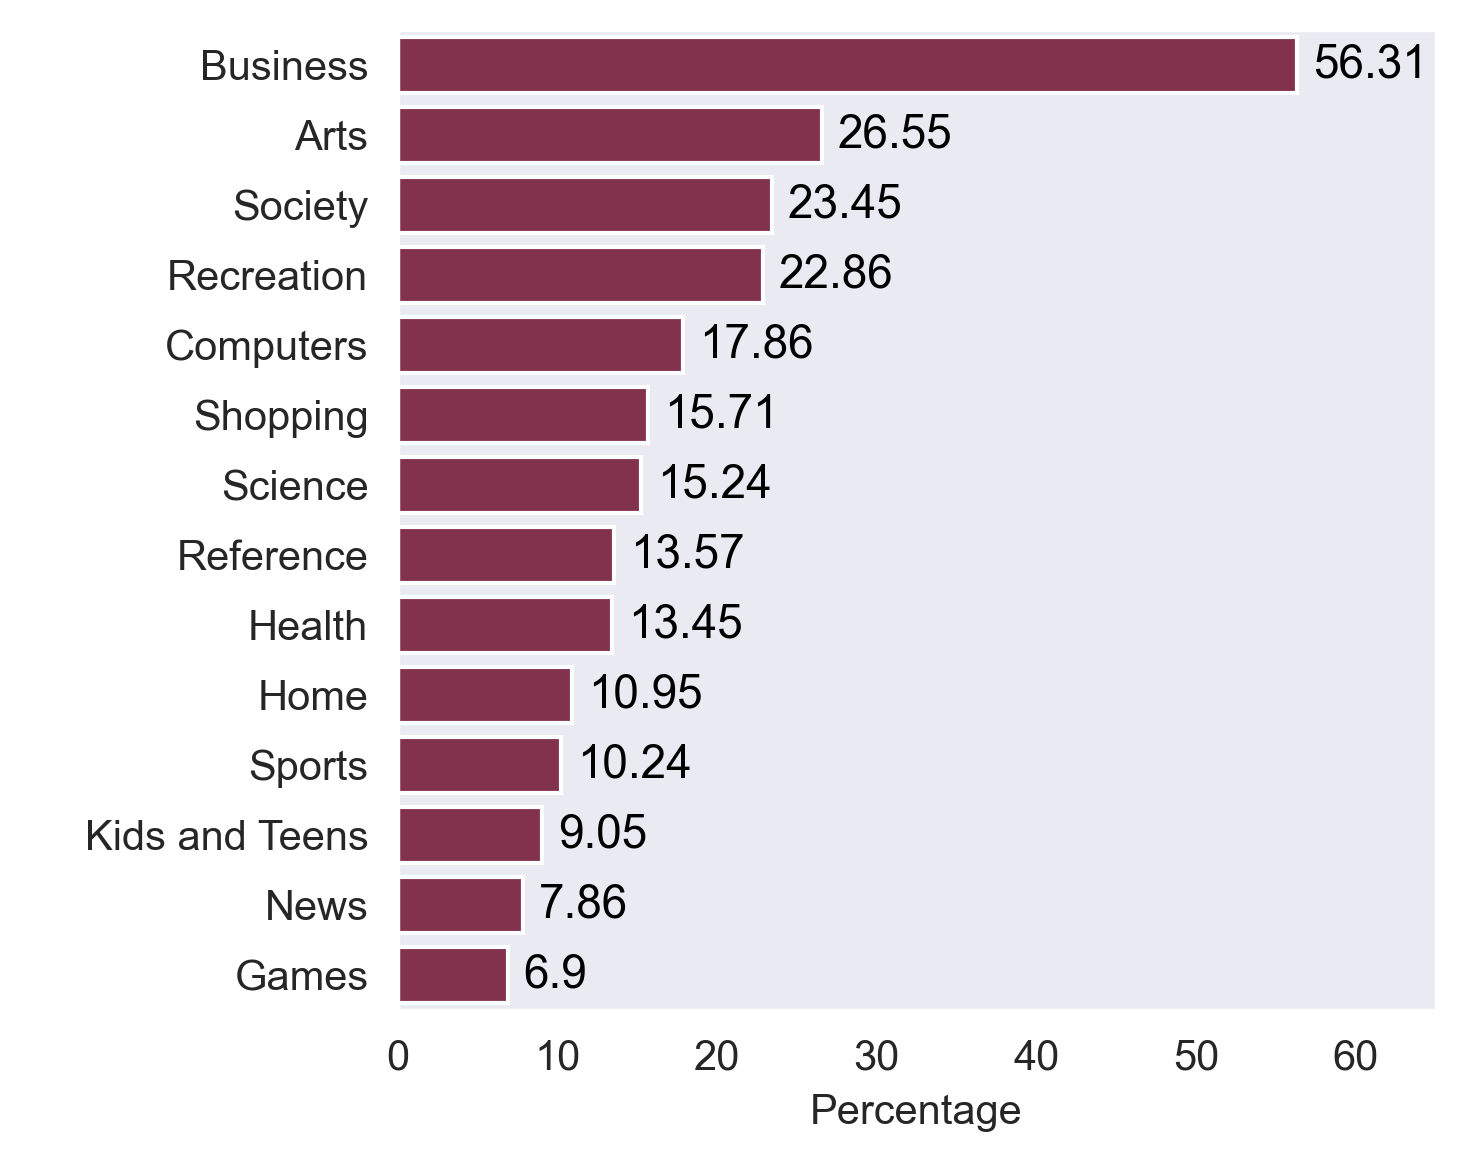
\includegraphics[width=1\columnwidth]{figures/category_distribution.png}
    \caption{Class distribution of the original dataset.}
    \label{fig:class_distribution}
\end{figure}

Figure \ref{fig:class_distribution} illustrates the class distribution of the original dataset. It is imbalanced, with most websites falling into the \textit{Business} category, followed by \textit{Arts} and \textit{Society}. This imbalance, identified in Homepage2vec, negatively impacted model performance on minority classes.
% 1. Step: Show that we can create high-quality annotations (measured against human annotations)
% - introduce curlie (talk about features (missing values), embedding, label list_ , re-scrape + process + embeddin
% ---> All this is pretty much in data, so transfer it here


% 2. Step: Show that we can improve performance compared to pre-trained model via fine-tuning with GPT annotations
% - training parameters (hparams, train/ test data splits)
% - evaluation procedure (macro f1, …)
% - calibration (?)
% TODO: this
\subsection* {Phase 2: Fine-Tuning the Baseline Model}
In the second phase, we fine-tune the baseline model with the obtained annotations from the \texttt{curlie-10k} dataset. And using the crowdsourced data as the test and validation set with 0.7/0.3 split.
We also perform a hyperparmeter search to find the best hyperparameters for the fine-tuning process. 
For this we employ Baeysian TPE samplerer from Optuna \cite{optuna} to efectively search the hyperparam space. 
The hyperparam values are detailed in Table \ref{tab:hyperparameters}.
\begin{table}[!ht]
    \centering
    \caption{\textbf{Hyperparameter Search Space}}
    \label{tab:hyperparameters}
    \begin{tabular}{ll}
    \toprule
    \textbf{Hyperparameter} & \textbf{Search Space} \\
    \midrule
    Learning Rate (\( \lambda \)) & $[0.00001, 0.01]$ \\
    Weight Decay (\( \beta \)) & $[0, 0.1]$ \\
    Scheduler Factor (\(\gamma\)) & $[0.1, 0.5]$ \\
    Batch Size (\(\delta\)) & \{64, 128, 256\} \\
    \bottomrule
    \end{tabular}
\end{table}


The best performing model is chosen by performance on the validation set using the multi-label macro F1 score, which is the average of the F1 score of each class. 
This model is then evaluated on the held out test set using macro F1, precision, recall, and accuracy.


